\section{Two-endpoint degeneration and the connecting return}
\label{sec:two-endpoints}

Suppose the limiting polynomial has a simple zero at each end of the
segment of equilibria. For nonnegative forcing, the long stay near the
left endpoint makes the complete-period multiplier smaller than one;
the attracting-annulus argument then bounds the number of cycles by two.
For negative forcing, the lower passage produces strong contraction and
a negative displacement. The intervening passage can amplify derivatives,
especially when the positive saddle has a small characteristic ratio.
We retain the contraction and signed displacement through this passage
and use the flat source of the resulting return map to bound its zeros.

\begin{proposition}\label{prop:two-endpoints}
Suppose
\[
 P_*(z)=C_*z^2-A_*z,\qquad C_*<0,\quad A_*>0,
 \qquad C_*f_{b_*}=A_* .
\]
Write the normalized forcing as $\delta=\varepsilon^3D$. There are
neighborhoods of $b_*$ and $(P_*,D=0)$, and positive constants
$\varepsilon_0,\rho$, such that the normalized family has total actual
minimal-return multiplicity at most two for isolated cycles at Hausdorff
distance less than $\rho$ from $\Gamma_0^b$
for $0<\varepsilon<\varepsilon_0$.
For every field in this neighborhood with $D\ge0$, there are at most two
cycles and each counted cycle is hyperbolic attracting; for $D<0$ there are at most two.
\end{proposition}

Throughout this section we write the nearby family exactly as
\begin{equation}\label{eq:lower-family}
 F=y(1+bz-y)+\varepsilon^2P(z),\qquad
 G=zy+\delta,\qquad
 P(z)=Cz^2-Az+A^2c,
\end{equation}
where $0<A_0\le A\le A_1$, $C$ belongs to a compact negative interval,
$c$ is small, and $\delta=\varepsilon^3D$. All constants are uniform
on a sufficiently small compact neighborhood of the limiting direction.
The sections in Lemma~\ref{lem:sections} will be kept fixed. In
particular, every cycle under consideration lies in $y>0$ and has a
unique intersection with the same outgoing section $z=z_c>0$.

For $D<0$, Lemma~\ref{lem:lower-saddle-transition} writes the lower
passage as a strong power followed by a contracting signed map.
Lemma~\ref{lem:lower-positive-references} constructs outgoing orbits of
the same field; their continuation to the physical section controls the
source derivatives in the return map. Proposition~\ref{prop:complete-signed-connector}
then continues the full signed power-output interval to the positive
saddle. It preserves the negative baseline
\eqref{eq:lower-negative-offset} and uses the lower contraction to absorb
intermediate growth, giving the weighted bounds
\eqref{eq:lower-connector-C2}. These are the inputs to
Lemma~\ref{lem:flat-two-saddle-comparison}.

Figure~\ref{fig:two-saddle-connector} records this composition.
There $\eta_0$ is the fixed incoming-cut height and $R>1$ is the lower-saddle
power exponent. The coordinate $a$ is the outgoing stable amplitude at the
positive saddle, $q=C_+(a)$ is its coordinate on the common physical section,
and $u(a)=u(C_+(a),p)$ is the corresponding lower-saddle source coordinate.
The quantity $t=\eta_0u(a)^R$ is the strong power output, $\Psi$ is the
physical connector with value $H(a)$, and $\mathcal D$ is the positive-saddle
Dulac map compared with $a$.

% Schematic composition of maps in the two-endpoint return.
% Arrows are map order, not phase-plane trajectories.
\begin{figure}[H]
\centering
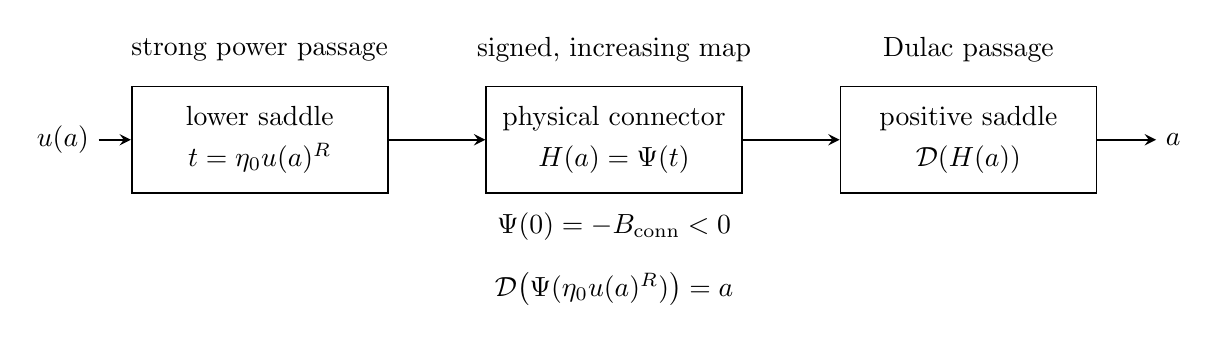
\begin{tikzpicture}[x=10mm,y=10mm,>=stealth,
  every node/.style={font=\fontsize{10}{12}\selectfont},
  block/.style={draw,line width=.6pt,minimum width=3.25cm,
    minimum height=1.35cm,align=center},
  map/.style={->,line width=.8pt}]
  \node (source) at (0,.2) {$u(a)$};
  \node[block] (lower) at (2.5,.2)
    {lower saddle\\[1mm]$t=\eta_0u(a)^R$};
  \node[block] (connector) at (7.0,.2)
    {physical connector\\[1mm]$H(a)=\Psi(t)$};
  \node[block] (positive) at (11.5,.2)
    {positive saddle\\[1mm]$\mathcal D(H(a))$};
  \node (target) at (14.1,.2) {$a$};
  \draw[map] (source)--(lower);
  \draw[map] (lower)--(connector);
  \draw[map] (connector)--(positive);
  \draw[map] (positive)--(target);
  \node at (2.5,1.35) {strong power passage};
  \node at (7.0,1.35) {signed, increasing map};
  \node at (11.5,1.35) {Dulac passage};
  \node at (7.0,-.9) {$\Psi(0)=-B_{\rm conn}<0$};
  \node at (7,-1.7)
    {$\mathcal D\!\left(\Psi(\eta_0u(a)^R)\right)=a$};
\end{tikzpicture}
\caption{Schematic composition of the complete negative-forcing two-endpoint return.
The arrows show the order of scalar maps, not phase-plane trajectories.
The full signed connector $\Psi$, with $\Psi(0)=-B_{\rm conn}<0$, is retained
in $H(a)=\Psi(\eta_0u(a)^R)$. The positive-saddle Dulac map is used on the
returning domain $H(a)>0$.}
\label{fig:two-saddle-connector}
\end{figure}


\subsection{Nonnegative forcing}

We prove attraction by estimating the complete-period multiplier.
The annulus count then gives the bound two.

Let $\mathfrak m$ be the characteristic multiplier of a positive cycle.
Since $z=(\log y)^{\boldsymbol\cdot}-\delta/y$, integration of the
divergence over a complete period gives the exact identity
\begin{equation}\label{eq:lower-multiplier}
 \log\mathfrak m
 =\oint\left[by-\varepsilon^2A
                  -(1+2\varepsilon^2C)\frac{\delta}{y}\right]dt.
\end{equation}
For $\delta\ge0$ the integrand is at most $by-\varepsilon^2A$.
The time spent near the left zero will dominate all positive contributions.
We estimate this time along the orbit, allowing reversals in $z$.

Choose fixed small $q,z_c,h_c>0$ such that the contact rectangle
$[-q,z_c]\times(0,h_c)$ satisfies
\begin{equation}\label{eq:lower-contact-box}
 1+bz-y\ge\tfrac12,\qquad F_y>0,\qquad P(-q)>p_q>0,
 \qquad |P(z)|\le A/(8b_+),
\end{equation}
where $b_+$ is an upper bound for $b$. The last two inequalities hold
after shrinking the coefficient neighborhood. The regular fast arc and
the descending passage to $y=K\varepsilon^3$ have uniformly bounded
positive contribution to \eqref{eq:lower-multiplier}. Indeed, on a fixed
negative interval, $G\le-c_0y$ for $y\ge K\varepsilon^3$, so a descent
from a fixed height $y_h$ contributes at most
$(b_+/c_0)\int_{K\varepsilon^3}^{y_h}dy$. The moving-entry estimate \eqref{eq:relaxation-map} gives
$\Lambda=\ell_b+O(\varepsilon^2(1+|\log\varepsilon|))$,
where $\ell_b$ is the regular fast-foot map.

Choose $H\ge K$ with $qH>\sup D$. Until the first subsequent hit of
$z=-q$, the boundary $y=H\varepsilon^3$ points downward. Thus the
positive cycle has $y\le H\varepsilon^3$ on this entire part of its
orbit, and the integrand in \eqref{eq:lower-multiplier} is at most
$-A_0\varepsilon^2/2$. This hit exists, since the same periodic orbit
must return to its upper fast section.

Put $f_*=f_{b_*}$ and fix $a>0$ with $f_*+a<-q$. For any sufficiently
small fixed $\tau>0$, shrink the coefficients and the fast source interval
so that $|\Lambda-f_*|\le\tau$ and
\[
 |P(z)|\le M(z-f_*+\tau)
       \quad(f_*+2\tau\le z\le f_*+a).
\]
Here $M$ can be chosen before $\tau$, since $P_*(f_*)=0$ and the
polynomial derivatives are bounded. Along the low orbit,
$|F|\le M\varepsilon^2(z-f_*+\tau+\varepsilon)$ on this strip.
To bound the crossing time even when $z$ reverses, use the function which equals
\[
 \log\frac{z-f_*+\tau+\varepsilon}{3\tau+\varepsilon}
\]
on the strip and is constant on each complementary half-line. Its
absolute time derivative is at most $M\varepsilon^2$. Its net change
between the descending entry and the first $-q$ hit is
$\log[(a+\tau+\varepsilon)/(3\tau+\varepsilon)]$. Consequently the
contribution of this whole low part is at most
\begin{equation}\label{eq:lower-log-time}
 -\frac{A_0}{2M}\log\frac{a}{4\tau},\qquad
 \varepsilon\le\tau.
\end{equation}
Leftward excursions do not affect this estimate: the function is constant
outside the strip, and its time derivative was estimated in absolute value.

At the first $-q$ hit the orbit enters the contact rectangle with
$F>0$. Its boundary clearances, positivity and $F_y>0$ give the
prescribed right exit with $F>0$ throughout, by the invariant-quadrant
argument in the proof of Lemma~\ref{lem:sections}.

Below $y_{\rm th}=\varepsilon^2A/(2b_+)$ the integrand of
\eqref{eq:lower-multiplier} is nonpositive. Above this height,
\eqref{eq:lower-contact-box} gives $F\ge y/4$. Its positive contact
contribution is therefore at most $4b_+(q+z_c)$. Fix all these positive
costs first, and then choose $\tau$ so that
\eqref{eq:lower-log-time} is smaller than their negative sum minus one.
Only afterward shrink the coefficients, source interval and
$\varepsilon_0\le\tau$. We obtain $\log\mathfrak m<-1$ for every
counted cycle, uniformly in all ratios of $c,D,\varepsilon$.
Choose $\mathcal A_-\Subset\mathcal A_+$ as in
Section~\ref{sec:graphic-anchored-annulus}, putting the larger annulus
inside the multiplier and section clearances and the counted cycles
and their intervening annuli in the smaller one. The estimate holds
throughout the ambient coefficient window for $D\ge0$.
Section~\ref{sec:ambient-genericity-window} supplies nondegenerate
perturbations with $D>0$, also from $D=0$. Lemmas~\ref{lem:equilibria}
and~\ref{lem:generic-attracting-index} now give the bound two.

\subsection{The lower passage for negative forcing}

The lower weak separatrix lies below $y=0$ for negative forcing.
We construct the transition from this negative baseline across the whole
power-output interval, with the first and second source derivatives
needed for the return comparison.

Assume henceforth that $\delta=-\nu<0$. At $y=0$ we have $G=-\nu$;
a trajectory which leaves $y>0$ cannot reenter it. This elementary sign
will also determine the displacement in the connection between the two
saddles.

Write $\mu:=\varepsilon^2$ for the slow scale and $\nu:=|\delta|$ for the
forcing magnitude. Below, $q$ is the physical ordinate on the outgoing
section, $u$ is the regular source coordinate, and $v$ is the normal
amplitude after the lower saddle passage.

\begin{lemma}\label{lem:lower-saddle-transition}
Let $q$ denote the physical ordinate on the outgoing section $z=z_c$;
we work on a fixed compact source interval in $q$, with the field
parameters $p$ held fixed.
Fix a small negative section $z=-q_0$ to the right of the lower polynomial
root. There are a regular source coordinate $u=u(q,p)$ and fixed
constants $\eta_0>0$, $0<\theta<1$, such
that every counted cycle has $0<u<\theta$ and reaches $-q_0$ with
ordinate
\begin{equation}\label{eq:lower-exact-transition}
 Y(q)=\Psi_-(\eta_0u(q)^R),\qquad
 R\asymp\varepsilon^{-2}.
\end{equation}
Here $p$ denotes the frozen field parameters,
\begin{gather}
 0<c_u\le u_q\le C_u,\qquad |u_{qq}|\le C_u,
 \label{eq:lower-regular-source}\\
 \Psi_-(v)=\beta_-+\kappa_-v[1+E(v/\varepsilon^2,p)],
 \qquad -M\nu\le\beta_-\le-m\nu<0,
 \label{eq:lower-signed-map}\\
 e^{-M/\varepsilon^2}\le\kappa_-\le e^{-m/\varepsilon^2},
 \qquad E(0,p)=0,\qquad \|E\|_{C^1}\le M .
 \label{eq:lower-signed-jets}
\end{gather}
The last norm is in the displayed amplitude variable, on a fixed small
interval; no parameter derivative is asserted. The signed map is $C^2$
on the whole interval $0\le v\le\eta_0\theta^R$. Its positive
part is one source interval, possibly empty. On this interval, after
shrinking $\varepsilon_0$,
\begin{equation}\label{eq:lower-flat-output}
 0<Y,Y_q\le M\varepsilon^{-2}e^{-m/\varepsilon^2},
 \qquad Y_{qq}\ge0,\qquad
 \nu\le M e^{-m/\varepsilon^2}\theta^R .
\end{equation}
\end{lemma}

\begin{proof}
Let $\beta<0$ be the lower root, so that $P'(\beta)>p_0>0$.
Set $\mu=\varepsilon^2$, fix the required final order $j\ge8$, and
first construct the invariant graph with additional phase derivatives.
For $\nu>0$, the substitution $y=\nu\zeta$ gives
\[
 \dot z=\nu\zeta(1+bz-\nu\zeta)+\mu P(z),\qquad
 \dot\zeta=z\zeta-1.
\]
These polynomial equations extend regularly to $\nu=0$.
The physical graph is recovered by $h=\nu\zeta$, which degenerates at
that parameter value.
At $\mu=\nu=0$, the graph $\zeta=1/z$ on the fixed negative
interval is normally attracting with a fixed spectral gap. Embed this
interval in a fixed compact boundaryless base and extend the graph and
field there, using a cut-off independent of the frozen field parameters.
Writing $w=\zeta-1/z$, the extended critical field has
$\dot z=0$ and $\dot w=a_0(z)w$ on $w=0$, with
$a_0\le-\sigma<0$. For a fixed order $r\ge 2j+12$, on a common tube
and uniformly in the frozen parameters,
$\|\dot z\|_{C^r}+\|\dot w-a_0(z)w\|_{C^r}\le C(\mu+\nu)$.
The compact boundaryless graph therefore has zero tangential rate and a
uniform normal gap. After one common shrinking of the parameter box,
Fenichel's compact normally-hyperbolic persistence theorem,
\cite[Theorem~3, p.~215]{Fenichel1971}, gives a persistent invariant
$C^r$ graph $\zeta=k(z;\mu,\nu,p)$ in a common tube.
The differentiated-maximum argument in the proof of
Lemma~\ref{lem:pc-selected-graph} applies with transport size
$\mu+\nu$ and normal coefficient $a_0\le-\sigma<0$; reversing its
sign does not change the absolute-value estimate. With
$r\ge2j+12$ it yields
$\|k-z^{-1}\|_{C^{2j+11}}\le C_j(\mu+\nu)$ on the extended circle.
Restrict the graph to
the nested working interval, where the extension agrees with the original
field. At $\nu=0$ its physical reconstruction is $h=\nu k\equiv0$.
The invariance equation gives the quantitative estimate:
\[
 zk-1=k_z\{\nu k(1+bz-\nu k)+\mu P(z)\}.
\]
Thus $k-z^{-1}=O_{C^{2j+10}}(\mu+\nu)$ and $h=\nu k$ satisfies
\begin{equation}\label{eq:lower-slow-graph}
 h(z)=\nu\{z^{-1}+O_{C^{2j+10}}(\mu+\nu)\},
 \qquad h<0\ \text{for }\nu>0,
\end{equation}
with the regular limiting choice $h\equiv0$ at $\nu=0$. Only phase derivatives, with the field fixed,
are used below. Notice also that $\nu/\mu=\varepsilon|D|\to0$
already follows from the normalization; it does not require the later
exponentially small survival estimate.

Translate the chosen graph by $w=y-h(z)$ and put
$q_n(z,w)=1+bz-2h(z)-w$. The exact equations are
\[
 \dot z=\mu\mathcal V(z)+q_n(z,w)w,\qquad
 \dot w=(z-h_zq_n(z,w))w,\qquad
 \mathcal V=P+\frac{h(1+bz-h)}\mu.
\]
The coefficients have common $C^{2j+8}$ bounds,
$\mathcal V=P+O_{C^{2j+8}}(\nu/\mu)$,
and the normal coefficient is bounded above by a negative constant.
Lemma~\ref{lem:uniform-normal-product} applies with $\tau=\mu$ and
$\rho=1$, at order $j+1$. It gives an exact product, preserving this particular graph,
with uniformly transverse normal coordinate.

The equilibrium on this graph lies at $z=\beta+O(\nu/\mu)$ and
has a negative eigenvalue bounded away from zero and a positive eigenvalue
comparable with $\mu$. The graph through it agrees to its right with
its weak unstable separatrix. Since $\mathcal V'$ is a positive unit at its
simple zero, the scalar change following
Lemma~\ref{lem:uniform-normal-product}, after division by the absolute
normal rate, gives
\begin{equation}\label{eq:lower-product}
 \dot\xi=\mu b_w\xi,\qquad\dot\eta=-\eta,\qquad 0<m_w<b_w<M_w .
\end{equation}
The coordinate $\xi$ increases to the right of the equilibrium.
This is an exact finite-order orbital normal form; its construction
does not divide by the small eigenvalue.

Choose the incoming cut $\eta=\eta_0>0$ and an outgoing weak cut
$\xi=\xi_{\rm out}>0$. The regular fast orbit reaches the incoming
cut in bounded time. Its weak coordinate, divided by $\xi_{\rm out}$,
is $u(q)$. The Poincar\'e determinant formula gives
\eqref{eq:lower-regular-source}, with positive orientation in physical
ordinate $q$: both transverse determinants are positive. After fixing
both weak exits, shrink the source so that their normalized absolute
incoming coordinate is less than $\theta<1$. The right local output is
exactly $v=\eta_0u^R$, with $R=(\mu b_w)^{-1}$.
For $u=0$ the orbit approaches the saddle below $y=0$. For $u<0$ its
left output is at most $\eta_0\theta^R$. Choose a fixed physical line
$z=z_{\rm left}$ left of all lower roots, with
$P(z_{\rm left})<-p_{\rm left}<0$. The still-positive left output has
height $o(\mu)$ there. For a small fixed $h_{\rm left}>0$, the half-strip
$z\le z_{\rm left}$, $0<y\le h_{\rm left}\mu$ has inward flow on its
right and upper sides. It cannot return to the positive outgoing section.

We next transfer the weak outgoing cut to a fixed physical vertical
section $z=z_l$, retaining the derivative loss caused by the slow speed.
Write the inverse coordinates as
$(z,y)=(X(\xi,\eta),H(\xi,\eta))$ and choose
$X(\xi_{\rm out},0)=z_l$. The nearby occurrence on that physical line
is determined by
\[
 X(\xi_{\rm out}e^{\mu b_wt},ve^{-t})=z_l.
\]
For $0\le v\le c_0\mu$, with $c_0>0$ fixed and small, its time derivative
is comparable with $\mu$. The normal direction is uniformly transverse,
and the weak exit stays a fixed distance from the base root. The
$\rho=1$ section change \eqref{eq:uniform-physical-section}, with
$v=\mu V$, therefore gives
\begin{equation}\label{eq:lower-cut-change}
 \Phi(v)=h(z_l)+a_lv+(v^2/\mu)E_l(v/\mu),\qquad
 a_l=H_\eta-h_zX_\eta>0,\qquad \|E_l\|_{C^{j-3}}\le M.
\end{equation}
In particular $\Phi'$ is bounded above and below by positive constants,
and $\Phi''/\Phi'=O(\mu^{-1})$. The actual argument range
$v\le\eta_0\theta^R$ is exponentially smaller than $\mu$.

On $[z_l,-q_0]$ the polynomial is uniformly positive. The signed tube
about $h$ has $F\asymp\mu$. For the scalar equation
$y_z=\mathcal R(z,y)=(zy-\nu)/F$,
\begin{equation}\label{eq:lower-scalar-derivative}
 \mathcal R_y=
 \frac{z(y^2+\mu P)+\nu(1+bz-2y)}{F^2},\qquad
 -M/\mu\le\mathcal R_y\le-m/\mu,
\end{equation}
and $|\partial_y^j\mathcal R|\le M_j\mu^{-j}$ for $j\ge2$.
Positivity at the lower right cut requires $\nu\le M\theta^R$, in
addition to $\nu/\mu\to0$. To define the transition also for signed
inputs, use the estimate on $\mathcal R_y$: it makes the tube
$|y-h(z)|\le c_1\mu$ forward invariant, for fixed small $c_1>0$.
After decreasing $c_0$, it contains the image of $\Phi$ on
$0\le v\le c_0\mu$. Thus the signed transition is defined on this whole
interval, not only on the exponentially short range of counted orbits.
Write its scalar part as $y(z,w)$ with $y(z_l,w)=w$, and put
$J=y_w$ and $L=(\log J)_w$. Their variational equations are
\begin{equation}\label{eq:lower-relative-variations}
 (\log J)_z=\mathcal R_y,\qquad L_z=\mathcal R_{yy}J,
 \qquad J(z_l)=1,\quad L(z_l)=0.
\end{equation}
Since $0<J\le e^{-m(z-z_l)/\mu}$, integration gives
$|y_{ww}/y_w|=|L|\le M\mu^{-1}$.
Composition with \eqref{eq:lower-cut-change} yields
$|\Psi_-''/\Psi_-'|\le M\mu^{-1}$.
Its baseline is $\beta_-=h(-q_0)$, between two fixed negative multiples
of $\nu$, and \eqref{eq:lower-scalar-derivative} gives the stated
exponential bounds for $\kappa_-=\Psi_-'(0)$. Moreover
$\Psi_-'(v)/\kappa_-$ is bounded above and below on $0\le v\le c_0\mu$.
For $V=v/\mu$, the exact formula
\[
 E(V,p)=\int_0^1
       \left\{\frac{\Psi_-'(t\mu V)}{\kappa_-}-1\right\}dt
\]
therefore gives $E(0,p)=0$ and a uniform $C^1$ bound on $0\le V\le c_0$.
This proves
\eqref{eq:lower-signed-map}--\eqref{eq:lower-signed-jets}.

The map $\Psi_-$ is increasing. Positivity at its target is equivalent
to positivity throughout the preceding orbit, because $G(z,0)<0$.
Hence $Y>0$ selects one upper interval and implies the last inequality
of \eqref{eq:lower-flat-output}. Finally, with $v=\eta_0u^R$,
\[
 \frac{Y_{qq}}{Y_q}
  =(R-1)\frac{u_q}{u}+\frac{u_{qq}}{u_q}
           +\frac{\Psi_-''}{\Psi_-'}R v\frac{u_q}{u}.
\]
The last term is bounded by $M R(v/\mu)u_q/u$ and is absorbed by the
first term on the whole interval. This proves convexity and the remaining
bounds in \eqref{eq:lower-flat-output}.
\end{proof}

\subsection{Positive outlets and local passages}

We first exclude contact constants bounded away from zero on the
negative scaled side, then treat the saddle-node range. For the remaining
positive outlets we construct reference orbits of the same field.
Their continuation to the physical section supplies the source derivative
bounds used in both the saddle-node and two-saddle returns.

Set
\begin{equation}\label{eq:lower-contact-parameters}
 k=\frac{c}{\varepsilon^2},\qquad
 \ell=-\frac{\nu}{A^3\varepsilon^6}.
\end{equation}
The survival inequality in \eqref{eq:lower-flat-output} implies
$\ell\to0$ uniformly whenever a counted cycle exists. For any fixed
$k_0>0$, the fields with $k\le-k_0$ have no such cycle. Indeed, on
the line $z_g=Ac/2<0$,
\[
 P(z_g)=A^2(c/2+Cc^2/4)\le-A^2|c|/4.
\]
At heights $0\le y\le h_g=A^2\varepsilon^2|c|/16$ the field points
left. Since $h_g\ge A_0^2k_0\varepsilon^4/16$, the output of
Lemma~\ref{lem:lower-saddle-transition} lies below this height for small
$\varepsilon$. The strip $z\le z_g$, $0<y\le h_g$ also points
inward on its upper side, and a downward exit cannot be reversed. This
argument includes $k\to-\infty$.

For $|k|$ small put $n=A\varepsilon^2$, $z=nU$, $y=n^2V$.
The exact equations are
\begin{equation}\label{eq:lower-epsilon-equations}
 U'=V(1+bnU-n^2V)+k-U+C\varepsilon^2U^2,\qquad V'=UV+\ell .
\end{equation}
Fix a small $d_0>0$, and choose $|k|\le k_c<d_0/8$ and
$|C|q_0\le A_0/8$. Then
\[
 P(-x)\ge\tfrac34 Ax,\qquad d_0A\varepsilon^2\le x\le q_0.
\]
Every still-positive lower output decreases in height while $z<0$.
It is exponentially smaller than $\varepsilon^2P$ down to $U=-d_0$,
so $F\ge\varepsilon^2P/2>0$ there. It either reaches this section
in finite time or first hits $y=0$. In the former case its ordinate and
first derivative in the scaled coordinate satisfy
\begin{equation}\label{eq:lower-central-small-entry}
 V=o(1),\qquad
 0<V_q\le M\varepsilon^{-6}e^{-m/\varepsilon^2}
       =:\zeta_\varepsilon\longrightarrow0,\qquad V_{qq}\ge0.
\end{equation}
Here convexity is preserved on the small negative tail. Indeed, direct
differentiation gives, with $Q=1+bz$,
\[
 \mathcal R_{yy}
 =\frac{2\{z[y^3+(3y-Q)\varepsilon^2P]
       -\nu[\varepsilon^2P+Q^2-3Qy+3y^2]\}}{F^3}>0,
\]
whereas $\mathcal R_y<0$ by \eqref{eq:lower-scalar-derivative}.
The forcing term is absorbed because
$\nu/(|z|\varepsilon^2P)\le M\nu\varepsilon^{-6}\to0$.
Only this small contact interval, where $Q>0$, is assigned a convexity
sign; the remote negative interval was included in $\Psi_-$.

Apply the finitely differentiable product coordinates of
Lemma~\ref{lem:saddle-node-passage} to \eqref{eq:lower-epsilon-equations}.
Write them as $\dot s=W(s,p)$, $\dot w=-w$, with center value
$\sigma(p)$. At $k=\ell=0$ the strong line is $V=0$, and
$s=V\chi(U,V)$ with $\chi>0$. Consequently the entries in
\eqref{eq:lower-central-small-entry} have
\[
 3d_0/4<w<5d_0/4,\qquad |s-\sigma|\le M(V+|k|+|\ell|).
\]
The fixed strong cut $w=w_0=d_0/2$ is reached in time
$\log(w/w_0)$, bounded above and below by positive constants. Its
coordinate is an increasing $C^3$ function of $V$, with bounded
logarithmic curvature. Thus the complete map $N(q)$ from the original
physical section to this cut satisfies
\begin{equation}\label{eq:lower-central-complement}
 N_q>0,\qquad \sup N_q\le M\zeta_\varepsilon,\qquad
 N_{qq}/N_q\ge-M\zeta_\varepsilon .
\end{equation}

The next lemma supplies the reference graphs and transverse incidence
required by Lemma~\ref{lem:positive-transition}. Applying that transition
lemma then gives the outgoing estimates on a fixed relative neighborhood
of each reference.

\begin{lemma}\label{lem:lower-positive-references}
Choose the fixed physical section $z=z_c>0$ before the final parameter
shrinking.  For every field admitting a counted lower passage, the
following three outgoing orbits continue to $z=z_c$:
\begin{enumerate}
 \item the zero-stable-amplitude orbit from the right exit of the
       saddle-node product box, for $|k|\le k_c$;
 \item the outgoing unstable separatrix of the positive saddle, for
       $k\in[k_c,K_1]$;
 \item the outgoing unstable separatrix of the small-ratio saddle, for
       $e=\varepsilon/\sqrt c\le e_0$.
\end{enumerate}
After the corresponding compact local outlet change, put
$z=nU$, $y=n^2V$, with $n=A\varepsilon^2$ in the first two cases and
$n=Ac$ in the third.  Each reference is a graph $V=h(U)$ on a fixed
positive scaled section and satisfies, up to $z=z_c$,
\begin{equation}\label{eq:lower-positive-reference-bounds}
 c_h(1+U^2)\le h(U)\le C_h(1+U^2),\qquad
 \mathcal F(U,h)\ge c_Fh,
\end{equation}
where $\mathcal F$ is the horizontal component of the scaled field.
The local outgoing amplitude $a$ can be oriented so that on the initial
reference section
\begin{equation}\label{eq:lower-positive-reference-incidence}
 g(a):=\frac{V(a)}{h}-1,\qquad g(0)=0,\qquad
 0<c_g\le g'\le C_g,\qquad |g''|+|g'''|\le C_g.
\end{equation}
All constants are uniform on the stated ranges.  Thus the reference and
initial-incidence hypotheses of Lemma~\ref{lem:positive-transition}
hold in its applications below.
\end{lemma}

\begin{proof}
All three cases reduce, after the local outlet change, to
\begin{equation}\label{eq:lower-positive-reference-system}
 \dot U=\mathcal F(U,V)=VQ(U,V)+p(U),\qquad
 \dot V=UV+\ell_*,\qquad Q=1+bnU-n^2V.
\end{equation}
For the first two cases
\[
 p(U)=k-U+C\varepsilon^2U^2,\qquad
 n=A\varepsilon^2,\qquad \ell_*=-\nu/n^3,
\]
whereas in the small-ratio case
\[
 p(U)=e^2(1-U)+C\varepsilon^2U^2,\qquad
 n=Ac,\qquad \ell_*=e^3\eta=-\nu/n^3.
\]
The survival estimate \eqref{eq:lower-flat-output} implies
$\ell_*\to0$ in all three cases and $\eta\to0$ in the last, since the
denominators lose at most a fixed power of $\varepsilon$.  Fix a small
$\varrho>0$.  After choosing $z_c$ and then shrinking the parameters,
\begin{equation}\label{eq:lower-positive-reference-Q}
 1-\varrho\le Q\le1+\varrho
\end{equation}
whenever $0\le z\le z_c$ and $y\le C(n^2+z^2)$.
The upper barriers below give this height bound and close the first-exit
argument on the chosen physical rectangle.

At the saddle-node organizer $k=\ell_*=\varepsilon=0$, the outgoing
center graph satisfies
\[
 h_0(U)=U+U^2+O(U^3),\qquad
 \mathcal F(U,h_0)=U^2+O(U^3).
\]
Fix a small $\delta>0$ and choose the right product exit so that its
zero-stable-amplitude orbit reaches $U=\delta$.  Finite smooth dependence
of the product and section coordinates gives
\begin{equation}\label{eq:lower-central-reference-entry}
 \begin{aligned}
 h(\delta)&=\delta+\delta^2
       +O(\delta^3+|k|+|\ell_*|+\varepsilon^2),\\
 \mathcal F(\delta,h(\delta))&=\delta^2
       +O(\delta^3+|k|+|\ell_*|+\varepsilon^2).
 \end{aligned}
\end{equation}
Decrease the previously chosen $k_c$, if necessary, so that
$k_c\le\kappa_0\delta^2$, and then shrink $\varepsilon$ and the forcing.
For $m_0=1+\delta/4$, the line $L_1=m_0U$ starts below the reference.
Its exact inward-crossing expression is
\begin{equation}\label{eq:lower-central-reference-linear}
 \begin{split}
 (UL_1+\ell_*)-L_1'\mathcal F(U,L_1)
 =m_0\{&(1-C\varepsilon^2-m_0bn+m_0^2n^2)U^2\\
       &-(m_0-1)U-k\}+\ell_*>0,
 \end{split}
\end{equation}
for $U\ge\delta$.  A fixed sufficiently small
$L_2=\gamma(1+U^2)$ is also a lower barrier: at a first meeting,
\[
 (UL_2+\ell_*)-L_2'\mathcal F(U,L_2)
 \ge UL_2\{1-2\gamma(1+\varrho+|C|\varepsilon^2/\gamma)\}
       -|\ell_*|-2\gamma U|k|>0.
\]
A fixed sufficiently large $H_2=M(1+U^2)$ is an upper barrier, since
$\mathcal F(U,H_2)\ge H_2/2$ and, at a first upward meeting,
\[
 \frac{UH_2+\ell_*}{\mathcal F(U,H_2)}<H_2'.
\]
The two lower barriers give
\begin{equation}\label{eq:lower-central-reference-speed}
 \frac{\mathcal F(U,h)}h
 \ge1-\varrho-\frac1{m_0}
       -\frac{|k|}{m_0\delta}-\frac{|C|\varepsilon^2}{\gamma}
 \ge c_F>0.
\end{equation}
The barriers and positive speed prove
\eqref{eq:lower-positive-reference-bounds} in the saddle-node range and
continue the reference to $z=z_c$.
The product coordinates may be oriented at the organizer by
$s=V+O(2)$ and $w=V-U+O(2)$.  Increasing the outgoing amplitude is then
positively transverse to the flow; the Poincar\'e determinant formula
and the compact transition to $U=\delta$ give
\eqref{eq:lower-positive-reference-incidence}.

For $k\in[k_c,K_1]$, let $(U_s,V_s)$ be the positive saddle and let $h$
be its actual outgoing unstable separatrix.  Choose a new fixed
$\delta_b\ll k_c$.  Uniform hyperbolicity gives on $U=U_s+\delta_b$
\begin{equation}\label{eq:lower-bounded-reference-entry}
 h=(1+k)\delta_b+O(\delta_b^2+\varepsilon^2+|\ell_*|),\qquad
 \mathcal F=k\delta_b+O(\delta_b^2+\varepsilon^2+|\ell_*|).
\end{equation}
Put $m_1=1+k_c/2$ and $t=U-U_s$.  The line
$L_1=m_1t$ begins below $h$, and its exact crossing expression is
\begin{equation}\label{eq:lower-bounded-reference-linear}
 (UL_1+\ell_*)-L_1'\mathcal F(U,L_1)
 =m_1t[U+1-m_1Q]-m_1(k-U_s)
      -m_1C\varepsilon^2U^2+\ell_*.
\end{equation}
On the compact $k$-interval the first term has a fixed positive lower
bound proportional to $t(1+U)$; it absorbs all remaining terms after
the parameter shrinking.  The same parabolic lower and upper barriers
as above give
\[
 \gamma(1+U^2)\le h(U)\le M(1+U^2),\qquad
 \frac{\mathcal F(U,h)}h
 \ge1-\varrho-\frac1{m_1}
      -\frac{|k-U_s|}{m_1\delta_b}-\frac{|C|\varepsilon^2}{\gamma}
 \ge c_F.
\]
Continue first from the parameter-dependent line $U=U_s+\delta_b$ to a
fixed $U_0>K_1+2\delta_b$.  This is a uniformly transverse compact
transition, after which the barriers continue to $z=z_c$.
The saddle separatrices and these fixed section maps have common finite
derivatives; orienting the outgoing amplitude by the positive transverse
determinant proves \eqref{eq:lower-positive-reference-incidence}.

It remains to construct the small-ratio reference.  In the variables of
\eqref{eq:lower-small-ratio}, its selected local outlet is the actual
outgoing unstable separatrix.  Continue it by a bounded local map to the
fixed horizontal level $Y=d_1>0$, where $X$ lies in a fixed positive
compact interval and $e|\eta|\ll d_1$.  Using $Y$ as phase until
$Y=e^{-2}$, one has
\[
 \frac{dX}{dY}=\frac{e^2\mathcal F_s}{XY+e\eta},\qquad
 \mathcal F_s=Y(1+bnX-n^2e^2Y)+1-X+CcX^2.
\]
The initially positive $\mathcal F_s$ cannot first vanish: at such a
point the term containing $X_Y$ vanishes and
\[
 \frac{d\mathcal F_s}{dY}=1+bnX-2n^2e^2Y>\tfrac12.
\]
Moreover $XY+e\eta\ge cXY$ and
\[
 \frac{d(X^2)}{dY}
 \le Ce^2(1+Y^{-1})+Cce^2X^2/Y.
\]
Gronwall's inequality gives positive uniform upper and lower bounds for
$X$ at $Y=e^{-2}$.  In the common variables this is the fixed horizontal
level $V=e^2Y=1$.  Continue to a fixed $U_0$ to its right; on that compact
piece $\mathcal F$ and $UV+\ell_*$ are positive units.  For $U\ge U_0$,
the barriers $\gamma(1+U^2)$ and $M(1+U^2)$ give
\[
 \gamma(1+U^2)\le h(U)\le M(1+U^2),\qquad
 \frac{\mathcal F(U,h)}h
 \ge1-\varrho-\frac{e^2U}{\gamma(1+U^2)}
             -\frac{|C|\varepsilon^2}{\gamma}\ge c_F.
\]
This proves \eqref{eq:lower-positive-reference-bounds} in the third case.

Finally orient its local amplitude so that increasing $a$ decreases the
outlet $X$ by a positive unit.  The $Y$-phase map has positive-unit first
variation and bounded derivatives through order three, since the relevant
coefficients have the integrable majorant $Ce^2(1+Y^{-1})$.  If $x(a)$
is the abscissa at $V=1$, then $x'(a)<-c<0$.  Differentiating the scalar
flow from this moving initial point to fixed $U_0$ gives
\[
 \partial_xV(U_0;x)
 =-\frac{x+\ell_*}{\mathcal F(x,1)}
   \exp\left(\int_x^{U_0}\partial_V
       \frac{UV+\ell_*}{\mathcal F(U,V)}\,dU\right)<0.
\]
All factors are positive units; hence $V_a(U_0)>0$ is a unit, and the
first three differentiated equations give
\eqref{eq:lower-positive-reference-incidence}.
As the scale and coefficient parameters approach the organizer, the
three references and their fixed relative collars converge on compact
subsets of $0<z\le z_c$ to its outgoing fast orbit. The small-ratio limit
here includes $c\to0$; for fixed nonzero small $c$, the fast limit may
start at the displaced positive root. In the joint limit the parabolic
bounds give zero height at $z=0$, and uniqueness for the regular fast
scalar equation identifies the limit. Thus, after first making the
coefficient neighborhood small enough, all references and collars reach
the same fixed transverse target inside its regular physical flow box.
This supplies the common target and its positive clearance for the return
construction.
\end{proof}

\paragraph{The saddle-node return.}
Return to the saddle-node passage and choose the right product exit
$s=s_+$ with $W(s_+)>0$.
The only entries which reach it have $[s,s_+]\subset\{W>0\}$;
they form one interval, to the right of the last root if roots are present.
The local map and its exact differential identity are
\begin{equation}\label{eq:lower-node-map}
 \mathcal D(s)=w_0\exp\left[-\int_s^{s_+}\frac{d\tau}{W(\tau)}\right],
 \qquad W\mathcal D'=\mathcal D .
\end{equation}
Let $C_+(a)$ be the continuation from this exit to the physical section.
Part~(1) of Lemma~\ref{lem:lower-positive-references} verifies the actual
reference and its positive-unit incidence.  Lemma~\ref{lem:positive-transition}
therefore gives $C_+'>0$ and bounded
$C_+''/C_+'$ and $C_+'$. For $H=N\circ C_+$,
\[
 aH''/H'\ge-Ma-Ma\zeta_\varepsilon\ge-M_1a.
\]
Fix the product box with $W_s\le1/4$, then $a_0$ with
$M_1a_0\le1/4$. The passage estimate in
Lemma~\ref{lem:saddle-node-passage} places every local output below
$a_0$ once its entry is sufficiently close to $\sigma$; choose $k_c$
and then $\varepsilon_0$ accordingly. Thus \eqref{eq:simple-pfaff-hypothesis} holds with margin $1/2$.
Lemma~\ref{lem:saddle-node-passage} gives total isolated return-zero
multiplicity at most two, including an exactly quadratic stationary zero.
The finite-passage domain is one interval, obtained from increasing maps:
positive lower output, positive entry at the strong cut, the unique
component of $W>0$ reaching $s_+$, and the original physical section
interval. The comparison therefore applies throughout this actual domain.

\paragraph{The positive Dulac map.}
We now prepare the positive-saddle passage for
Lemma~\ref{lem:flat-two-saddle-comparison}.
It suffices to consider fields admitting a counted cycle, so that the
survival bound in \eqref{eq:lower-flat-output} holds.
In the range $k\in[k_c,K_1]$, equation~\eqref{eq:lower-epsilon-equations}
gives a positive saddle with eigenvalues near $-1$ and $k$, and ordinate
$-\ell/U_s>0$. For large $k$, put
\begin{equation}\label{eq:lower-small-ratio}
 e=\varepsilon/\sqrt c,\quad n=Ac,\quad
 z=nX,\quad y=n^2e^2Y,\quad \eta=-\nu/(n^3e^3).
\end{equation}
Here $c\ge K_1\varepsilon^2$ and $A\ge A_0$, so the survival bound
implies $|\eta|\le M\varepsilon^{-6}e^{-m/\varepsilon^2}\to0$.
The equations become
\[
 X'=e^2\mathcal F,\quad
 \mathcal F=Y(1+bnX-n^2e^2Y)+1-X+CcX^2,\qquad
 Y'=XY+e\eta.
\]
The saddle near $(1,0)$ has characteristic ratio $r=e^2\beta_s$,
where $\beta_s$ is bounded above and below by positive constants.
Lemma~\ref{lem:small-ratio-saddle} applies with the present bounded
negative $C$ and the chosen stable graph. Its use of
Lemma~\ref{lem:uniform-normal-product} has $\tau=\rho=e^2$ and a
fixed positive normal gap, or a negative gap in reversed time. It gives
the exact $C^j$ orbital normal form
\begin{equation}\label{eq:lower-positive-product}
 \dot\xi=-r\xi,\qquad\dot\omega=\omega,\qquad
 \mathcal D(s)=\xi_0(s/\omega_0)^r.
\end{equation}
The stable graph is $Y=-e\eta/X+O_{C^j}(e^3|\eta|)>0$ and the
strong-fiber slope in $X$ is $O_{C^{j-1}}(e^2)$.


\subsection{The signed connector and the two-saddle return}

For $k\ge k_c>0$, the connector must carry the lower power output to the
positive saddle. When its characteristic ratio is small, this passage
can amplify height and derivatives by an exponential factor. The lower
contraction must dominate that factor on the whole signed input interval.
The next proposition proves this domination, preserves the negative
baseline, and bounds the weighted logarithmic curvature needed by
Lemma~\ref{lem:flat-two-saddle-comparison}.

\begin{proposition}[The complete signed connector]
\label{prop:complete-signed-connector}
Fix the compact coefficient window in \eqref{eq:lower-family}, the finite
phase order, and the selected lower graph and positive-saddle coordinates
constructed above. The lower weak unstable branch is the zero source;
the incoming unstable coordinate increases with physical height from
the positive saddle's stable branch. Fix $k_c>0$, a small-ratio threshold
$e_0>0$, and $K_1\ge\max\{k_c,e_0^{-2}\}$.
For each final choice of the lower power-output cut and compatible
canonical incoming cuts within the fixed saddle cores, take
$\eta_0>0$, $0<\theta<1$, $R\asymp\varepsilon^{-2}$ and the survival
constants $C_s,m_s>0$ from Lemma~\ref{lem:lower-saddle-transition} and
\eqref{eq:lower-flat-output}. There are $\bar c,\varepsilon_0>0$ such
that every field in this window satisfying
\[
 \delta=-\nu<0,\qquad
 0<\varepsilon<\varepsilon_0,\quad 0<c<\bar c,\quad
 k=c/\varepsilon^2\ge k_c,\qquad
 0<\nu\le C_s\theta^R e^{-m_s/\varepsilon^2}
\]
has the following connector. Put $t_*=\eta_0\theta^R$.
The forward flow from the entire lower power-output interval
$0\le t\le t_*$ reaches the selected canonical incoming section of the
positive saddle in finite positive time. Its unstable coordinate defines
$\Psi\in C^2([0,t_*])$ with
$\Psi(0)=-B_{\rm conn}<0$ and $\Psi'>0$, and
\begin{equation}\label{eq:lower-connector-C2}
 \eta_0\sup_{[0,t_*]}\Psi'\le1,\qquad
 \left|t\frac{\Psi''(t)}{\Psi'(t)}\right|\le1
 \quad(0<t\le t_*).
\end{equation}
The estimates are uniform for these fields; all source derivatives are
taken with the vector field fixed.
\end{proposition}

\begin{proof}
Continue the whole signed interval $0\le v\le\eta_0\theta^R$
from Lemma~\ref{lem:lower-saddle-transition} to the canonical incoming
section of the positive saddle. Put $\mu=\varepsilon^2$.
The signed lower transition and the assumed survival bound give, with
$0<\theta<1$,
\begin{equation}\label{eq:lower-connector-input}
 |Y(-q_0)|\le M(\theta^R+\nu),\quad
 \nu\le M\theta^R e^{-m/\mu},\quad R\ge r_-/\mu,
\end{equation}
where $Y(-q_0)=\Psi_-(v)$. On this $v$-interval,
$0<\Psi_-'(v)\le M e^{-m/\mu}$, and
$|\Psi_-''(v)/\Psi_-'(v)|$ is bounded
by a fixed power of $\varepsilon^{-1}$. With the finite phase order,
$e_0$, $K_1$, the saddle cores and root gap fixed, choose the cuts and
tube widths before the upper bound $\bar c$ for $c$. The restrictions
\begin{equation}\label{eq:lower-connector-geometry}
 LA_1\bar c<q_0,\qquad LA_1\varepsilon_0^2<q_0
\end{equation}
are imposed before shrinking $\varepsilon_0$.

Choose $q_0$ smaller, if necessary, so that
\begin{equation}\label{eq:lower-connector-P}
 P(-x)\ge \frac78Ax+A^2c\qquad(0\le x\le q_0).
\end{equation}
In the bounded-ratio range set $n=A\varepsilon^2$ and in the small-ratio
range set $n=Ac$.  Thus $n\ge c_n\varepsilon^2$.  With
\[
 \omega_\varepsilon=K\{\theta^R+\nu/n\},
\]
choose $K$ larger than twice the constant in
\eqref{eq:lower-connector-input}, and then require $LK>2$, $n<1$, and
$\omega_\varepsilon<1/2$.  Let $B_1,C_Q$ bound respectively
$|1+bz-y|$ and $|1+bz-2y|$ on the contact box.  Since the right side of
\eqref{eq:lower-connector-P} is bounded below by a fixed multiple of
$n$, polynomial losses in $\varepsilon^{-1}$ are dominated by the
exponential factors in \eqref{eq:lower-connector-input}; hence we may impose
\begin{equation}\label{eq:lower-connector-smallness}
 B_1\omega_\varepsilon\le \frac{\varepsilon^2}{4}
       \min_{Ln\le x\le q_0}P(-x),\qquad
 C_Q\nu\le \frac{x\varepsilon^2P(-x)}{4}
       \quad(Ln\le x\le q_0).
\end{equation}
For $z=-x$ and $|y|\le\omega_\varepsilon$, (\ref{eq:lower-connector-smallness})
therefore gives
\begin{equation}\label{eq:lower-connector-F}
 \frac12\varepsilon^2P(z)\le F(z,y)
 \le \frac32\varepsilon^2P(z).
\end{equation}
The upper horizontal face has $G=-x\omega_\varepsilon-\nu<0$, while the
lower face satisfies
\[
 G=x\omega_\varepsilon-\nu\ge xK\theta^R+(LK-1)\nu>0.
\]
Thus the signed interval reaches $z=-Ln$ inside this strip.  For
$\mathcal R=G/F$ an exact differentiation gives
\begin{equation}\label{eq:lower-connector-Ry}
 \mathcal R_y=\frac{z(y^2+\varepsilon^2P)+\nu(1+bz-2y)}{F^2}<0.
\end{equation}
If $J=y_{y_0}$ and $L_2=y_{y_0y_0}/J$, then
\begin{equation}\label{eq:lower-connector-variations}
 J_z=\mathcal R_yJ,\qquad (L_2)_z=\mathcal R_{yy}J.
\end{equation}
Since $0<J\le1$ and the coefficients of $\mathcal R$ are bounded by fixed
powers of $\varepsilon^{-1}$, integration bounds $L_2$ by such a power.
For the terminal map $H(y_0)=y(-Ln;y_0)$ and $g=H\circ\Psi_-$,
\[
 \frac{H''}{H'}=L_2,\qquad
 \frac{g''}{g'}=(L_2\circ\Psi_-)\Psi_-'
                         +\frac{\Psi_-''}{\Psi_-'}.
\]
Thus passage to the inner scale preserves exponential contraction of
the first derivative and introduces only polynomial growth in the
relative second derivative.

For $k\in[k_c,K_1]$, use $n=A\varepsilon^2$, $z=nU$, $y=n^2V$ and
$\ell=-\nu/(A^3\varepsilon^6)$. Write
\[
 F_b(U,V)=V(1+bnU-n^2V)+k-U+C\varepsilon^2U^2
\]
for the horizontal component of \eqref{eq:lower-epsilon-equations}.
On $[-L,0]$ and $[0,U_s-\sigma]$, where $U_s$ is its positive
zero at $V=0$, one has $F_b(U,0)\ge c_*>0$ after shrinking
$\varepsilon$.
Writing $D_\varepsilon=|V(-L)|+|\ell|$, a first-exit tube
$|V|\le K_{\rm Gr}D_\varepsilon$ (with $K_{\rm Gr}$ larger than the fixed
Gronwall constant)
closes because the $V$ contribution to $F_b$ is at most $c_*/2$.
The scalar equation and its first two $V$ derivatives are uniformly bounded
on this fixed interval; hence Gronwall and the analogous variational
recursions in \eqref{eq:lower-connector-variations} give
\begin{equation}\label{eq:lower-middle-bounded}
 0<\Psi'\le M\varepsilon^{-N}e^{-m/\varepsilon^2},\qquad
 \left|\frac{\Psi''}{\Psi'}\right|\le M\varepsilon^{-N}.
\end{equation}
The final passage to the canonical incoming cut is a compact hyperbolic
flow-box change with positive unit derivative and bounded $C^2$ jets.

It remains to treat $c\ge K_1\varepsilon^2$.  Put
\[
 e=\frac{\varepsilon}{\sqrt c},\quad n=Ac,\quad z=nX,
 \quad y=n^2e^2Y,
\]
so that
\begin{equation}\label{eq:lower-connector-small-system}
 X'=e^2\mathcal F,\qquad Y_X=\frac{XY+e\eta}{e^2\mathcal F},\qquad
 \mathcal F=Y(1+bnX-n^2e^2Y)+1-X+CcX^2,
\end{equation}
with $\eta=-\nu/(n^3e^3)$.  Decrease $\bar c$ so that, for a fixed
$\sigma>0$, $1-X+CcX^2\ge3c_\sigma$ on $[-L,1-\sigma]$; then choose
$\delta_0$ so that $\mathcal F\ge2c_\sigma$ whenever $|Y|\le\delta_0$.
At $X=-L$, the preceding strip estimate gives
\[
 |Y|+|\eta|\le M\varepsilon^{-N_0}e^{-a_0/\varepsilon^2}.
\]
On the provisional tube the first two $Y$ derivatives of the right side in
\eqref{eq:lower-connector-small-system} are bounded by $M/e^2$.
Gronwall gives a factor $\exp(M_*/e^2)$.  After these constants are fixed,
shrink $\bar c$ so that, with $a_\theta=r_-|\log\theta|$,
\begin{equation}\label{eq:lower-connector-exponents}
 M_{\rm ht}\bar c<a_0/3,\qquad M_*\bar c<m/3,\qquad
 M_*\bar c<a_\theta/3.
\end{equation}
These choices have three separate uses: the first closes the height
tube, the second preserves the lower-saddle decay of $\Psi'$, and the
third makes the curvature bound small after multiplication by $\theta^R$.
For $J=Y_{Y_0}$ and $L=Y_{Y_0Y_0}/J$, the exact equations
\[
 J'=f_YJ,\qquad L'=f_{YY}J
\]
with $f$ the right side of the scalar equation yield
\[
 J\le e^{M/e^2},\qquad |L|\le Me^{-2}e^{M/e^2}.
\]
Consequently, after the physical connector, the complete signed map satisfies
\begin{equation}\label{eq:lower-middle-small-ratio}
 0<\Psi'\le\varepsilon^{-N}e^{-m/\varepsilon^2+M_*/e^2},\qquad
 \left|\frac{\Psi''}{\Psi'}\right|
 \le\varepsilon^{-N}e^{M_*/e^2}.
\end{equation}

We finally make the section conversion explicit.  In finite-order product
coordinates near the positive saddle, write
\[
 \dot\xi=-r_s\xi,\qquad \dot\omega=\omega,\qquad
 r_s=e^2\beta_s,\qquad 0<\beta_-\le\beta_s\le\beta_+,
\]
with $-X_\xi\asymp1$ and $X_\omega=O_{C^2}(e^2)$ in the physical
coordinate $X=X(\xi,\omega)$.  Fix the canonical cut $\xi=\xi_b$ and
$T_0>0$, and set $x_v=X(\xi_be^{r_sT_0},0)$.  The preceding vertical cut is
specified by
\[
 X(\chi(\omega),\omega)=x_v,
\qquad \chi^{(j)}(\omega)=O(e^2),\quad 1\le j\le2.
\]
The canonical hitting time is
\[
 T(\omega)=r_s^{-1}\log \frac{\chi(\omega)}{\xi_b}.
\]
The common factor $e^2$ cancels in its first two derivatives.  Choosing
its fixed normal half-width $d$ so that
\[
 K_Xd<\tfrac14\beta_-\xi_bT_0,\qquad
 d\sup|T'|<\tfrac12,
\]
ensures positive hitting time and makes
$\omega\mapsto\omega e^{T(\omega)}$ increasing; a further fixed reduction
keeps its image in the canonical collar.  Since
\[
 Y=Y_s(\xi)+\omega u_1(\xi,\omega),\qquad u_1\ge u_*>0,
\]
we have on this vertical line
\[
 \frac{d}{d\omega}Y(\chi(\omega),\omega)=u_1+O(e^2)+O(d)>0,
\]
with bounded second derivative.  Thus conversion from physical
height to $\omega$, followed by the hitting map, is an increasing $C^2$
change preserving \eqref{eq:lower-middle-small-ratio}. The whole signed
input interval therefore reaches the canonical incoming cut in finite
time, with these estimates.


The baseline $v=0$ starts at the negative-height weak separatrix of the
lower saddle and stays negative, because $G(z,0)=-\nu<0$. The incoming
stable separatrix of the positive saddle lies in $y>0$: a nonpositive
point could not converge to its positive equilibrium. Physical height
on the incoming section increases with its unstable coordinate, whose
zero is this stable separatrix. Therefore
\begin{equation}\label{eq:lower-negative-offset}
 \Psi(0)=-B_{\rm conn}<0.
\end{equation}
This compares the two actual separatrices at the canonical target and
fixes the sign of the connector offset.

It remains to prove \eqref{eq:lower-connector-C2}. For these fixed final
saddle cuts, $t_*=\eta_0\theta^R$.
Equations~\eqref{eq:lower-middle-bounded} and
\eqref{eq:lower-middle-small-ratio}, with $1/e^2=c/\varepsilon^2$, give
\[
\begin{aligned}
 \eta_0\sup_{[0,t_*]}\Psi'
 &\le M\eta_0\varepsilon^{-N}
       e^{-(m-M_*\bar c)/\varepsilon^2},\\
 \sup_{0<t\le t_*}\left|t\frac{\Psi''}{\Psi'}\right|
 &\le M\eta_0\varepsilon^{-N}
       e^{-(a_\theta-M_*\bar c)/\varepsilon^2}.
\end{aligned}
\]
Here $M_*=0$ in the bounded-ratio range. After fixing the cuts,
choose $\bar c$ as in \eqref{eq:lower-connector-exponents} and then
shrink $\varepsilon_0$. These bounds give \eqref{eq:lower-connector-C2}
on the full signed input interval.
\end{proof}

\paragraph{The return equation and its zeros.}
Use the connector of Proposition~\ref{prop:complete-signed-connector}.
Let $a$ be the outgoing stable amplitude at the positive saddle.
Parts~(2) and~(3) of Lemma~\ref{lem:lower-positive-references} verify,
respectively, the bounded-ratio and small-ratio reference graphs and
their positive-unit incidence.  Lemma~\ref{lem:positive-transition}
therefore gives the positive physical
continuation $q=C_+(a)$, with
\[
 0<C_+'\le Mn^{3/2},\qquad
 |C_+''/C_+'|\le M.
\]
Together with \eqref{eq:lower-regular-source}, this implies that
$u(a):=u(C_+(a),p)$ satisfies
\[
 0<u_a\le Mn^{3/2},\qquad
 \frac{u_{aa}}{u_a}
 =\frac{u_{qq}}{u_q}C_+'+\frac{C_+''}{C_+'}=O(1).
\]
The exact complete complement is
\begin{equation}\label{eq:lower-complete-middle}
 H(a)=\Psi(\eta_0u(a)^R).
\end{equation}
The actual returning domain is the intersection of the fixed outgoing
amplitude interval, the inverse image of the physical source interval,
$0<u<\theta$ and $0<H<s_0$. It is one interval because all these maps
are increasing. The lower positivity condition is an upper interval;
it is already forced by $H>0$, since the target then lies above the
positive stable branch and no earlier negative height can reach it.

Every counted cycle has this passage. Its lower branch was selected in
Lemma~\ref{lem:lower-saddle-transition}, and the preceding estimates
keep its entire approach inside the positive saddle's incoming tube.
Starting at its positive $-q_0$ hit, the contact-rectangle argument above
again gives $F>0$ up to the outgoing physical section, using
$P(-q_0)>0$, $F_y>0$, positivity of the orbit and the boundary
clearances.
In the bounded-ratio saddle a negative unstable input leaves through the
left side with $F<0$, contradicting this contact speed; a zero input has
infinite flight time. In
\eqref{eq:lower-positive-product}, a negative normal input reaches
negative physical height before the fixed negative normal exit, whereas
a zero input is the stable separatrix. Only $s>0$ can complete the
required passage.

By Proposition~\ref{prop:complete-signed-connector}, on the actual
returning interval,
\[
 0<H=\Psi(t)<\Psi(t)+B_{\rm conn}
       =\int_0^t\Psi'(v)\,dv\le u^R.
\]
The lower product gives $R\le M\varepsilon^{-2}$, so
\[
 \begin{array}{ll}
 n=A\varepsilon^2:& R\sup u_a\le M\varepsilon,\\
 n=Ac,\quad r=e^2\beta_s:& Rr\sup u_a\le M\sqrt c.
 \end{array}
\]
The first bound controls $R\sup u_a$ in the bounded-ratio comparison;
the second controls $Rr\sup u_a$ in the small-ratio comparison. Together
with the bounded logarithmic curvature of $u$, they supply the source
hypotheses of Lemma~\ref{lem:flat-two-saddle-comparison}.

For bounded $k$, Lemma~\ref{lem:dulac-jets} supplies
\eqref{eq:lower-dulac-jets} uniformly through ratio one.
Moreover $H'=\eta_0\Psi'(t)Ru^{R-1}u_a$ tends uniformly to zero,
and $Rr\ge2$ for small $\varepsilon$. The second case of
Lemma~\ref{lem:flat-two-saddle-comparison} therefore gives at most two
return zeros.
For small $e$, \eqref{eq:lower-positive-product} is exact and
\[
 Rr\ge r_-\inf\beta_s/c\ge2
\]
after shrinking $\bar c$. Fix the outgoing normal cut $\omega_0$ and a
weak amplitude interval first, and bound the regular source derivatives
on that interval. The power prefactor
$c_D=\xi_0\omega_0^{-r}$ then has a fixed upper bound for $r\le r_0<1$
and for every subsequent choice of $\xi_0$ in this interval.
With this bound and $L_\Psi=1$, the first case of
Lemma~\ref{lem:flat-two-saddle-comparison} gives $a_0$ and $\eta_*$.
Keeping $\omega_0$ unchanged, choose the incoming weak cut $\xi_0\le a_0$
and a separate incoming normal interval of width
$d_{\rm in}\ll\xi_0$. Moving its preceding vertical cut by
$O(e^2d_{\rm in})$ gives a forward matching time
$O(d_{\rm in}/\xi_0)$. For these final cuts, apply
Proposition~\ref{prop:complete-signed-connector}: first shrink $\bar c$
as in \eqref{eq:lower-connector-exponents}, and then $\varepsilon_0$,
to obtain \eqref{eq:lower-connector-C2}. Every local output satisfies
$\mathcal D(s)\le\xi_0\le a_0$, and decreasing $\bar c$ also makes
$Rr\sup u_a\le M\sqrt c\le\eta_*$. The first case of the comparison
applies on the whole interval and gives the same bound two.
Section~\ref{sec:return-framework} identifies these simple or quadratic
zeros with the corresponding actual minimal-return multiplicities.

\begin{proof}[Completion of the proof of Proposition~\ref{prop:two-endpoints}]
The sign $D\ge0$ was treated by \eqref{eq:lower-multiplier}.
For $D<0$, the lower survival inequality supplies every required small
$\ell$ uniformly. Fix the central constant $k_c$ first. The three
alternatives $k<-k_c$, $|k|\le k_c$ and $k>k_c$ have bounds zero,
two and two, respectively. To cover the last alternative, obtain a
small-ratio threshold $e_0$ and choose the final finite
$K_1\ge\max(k_c,e_0^{-2})$; take the bounded-ratio constants on
this final interval $[k_c,K_1]$. The two alternatives overlap because
$e=1/\sqrt k$.
There are finitely many cuts, coefficient neighborhoods, and positive
$\varepsilon$ and Hausdorff thresholds; take a common shrinking
compatible with them. Each fixed field has one sign of $D$ and one
value of $k$. Thus every counted cycle of that field is controlled by
the same regional argument, and the maximum of the regional bounds
gives the bound on the whole coefficient neighborhood. Every sufficiently
close cycle has its unique physical section point in the selected source
interval by
Lemma~\ref{lem:sections}. This proves the proposition.
\end{proof}

\subsection{The common two-endpoint window}\label{sec:common-two-endpoint-window}
For a normalized direction $q=(E_0,E_1,E_2,D)\in S^3$ with
$E_1,E_2<0$, use the single chart
\[
 A=-E_1,\qquad C=E_2,\qquad c=E_0/A^2 .
\]
The limiting two-endpoint curve over $J$ is
\[
 q_b^*=(0,-A_b,C_b,0),\qquad
 A_b=-f_b/\sqrt{1+f_b^2},\quad
 C_b=-1/\sqrt{1+f_b^2}.
\]
It is compact and $A_b,-C_b$ have positive lower bounds.
The negative-forcing proof fixes its final central threshold,
small-ratio threshold, and bounded-ratio interval before choosing
the open coefficient window. The nonnegative proof fixes the
larger forcing bound, the bounds on all positive contributions, and the
logarithmic time tolerance before its strict joint window. Both windows
contain the same curve and use the same physical field and cores.

Pull the ambient nonnegative window back to the normalized chart
and intersect it with the negative window near each $q_b^*$.
Choose smaller balls with closed balls contained in these effective
intersections. Finitely many cover the limiting curve.
Their union contains a tube of positive radius about it, by
compactness. On their closures the two signs' terminal radial
and Hausdorff thresholds have a positive finite minimum.
This supplies one open two-endpoint window allowing
$Cf_b\ne A$, $c\ne0$, and both signs of $D$.
For a fixed field the sign selects one entire estimate;
the cycle bound is $\max(2,2)=2$.

